% !TEX program = pdflatex
% =============================================================================
% Sep 10 advisor meeting — first meeting since Aug 12 (Aug 26 did not happen).
% Arc: Aug-12 asks resolved -> what we built & measured (F1, RL on Nautilus) ->
% the two headline findings (training saves 32% energy; the effort knob is NOT
% yet a decision) -> the experiment matrix running right now -> asks.
% All numbers: 134 OOD ALFWorld games, per-board-calibrated energy, RTX 3090.
% =============================================================================
\documentclass[10pt,aspectratio=169]{beamer}

\usetheme{metropolis}
\usepackage{appendixnumberbeamer}
\usepackage{booktabs}
\usepackage{amsmath,amssymb}
\usepackage{xcolor}
\usepackage{hyperref}
\usepackage{graphicx}
\usepackage{tikz}
\usetikzlibrary{arrows.meta,positioning,fit}

\definecolor{good}{HTML}{1baf7a}
\definecolor{bad}{HTML}{e34948}
\definecolor{mid}{HTML}{eb6834}
\definecolor{acc}{HTML}{2a78d6}
\newcommand{\rf}[1]{{\scriptsize\textcolor{black!55}{[#1]}}}
\newcommand{\ab}[1]{\textless#1\textgreater}  % <tag> in the trace slide

\title{Effort as an action: what trained, what it learned, and what it refuses to learn}
\subtitle{Everything since Aug 12 --- baselines, RL on Nautilus, and the decision problem}
\author{Daniela Rojas}
\date{September 10, 2026}

\begin{document}
\maketitle

% =============================================================================
% MAIN DECK: 4 slides. Everything else lives in the appendix.
% =============================================================================
% -----------------------------------------------------------------------------
\begin{frame}{What we tried: let the agent choose how hard to think}
\small
Every turn, the agent writes one text with its choice, its reasoning, and its move:
\begin{center}
{\ttfamily\normalsize
\textcolor{mid}{\ab{effort}low $|$ mid $|$ high\ab{/effort}}\;
\textcolor{acc}{\ab{think}} \ldots \textcolor{acc}{\ab{/think}}\;
\textcolor{good}{\ab{action}} go to countertop 1 \textcolor{good}{\ab{/action}}}
\end{center}
\vspace{0.3em}
\begin{itemize}\itemsep 0.5em
  \item The game (ALFWorld) sees \textbf{only the action}. The effort tag is the agent's own
        declaration of how much reasoning to spend; a hardware counter measures the \textbf{joules}
        of every generated token.
  \item \textbf{The reward}: \; $R \;=\; 10\cdot\mathbf{1}[\text{success}]\cdot
        \max\!\big(0,\; 1-0.5\,E/E_{\text{ref}}\big)$ \; --- win, and win \emph{cheaply}.
  \item \textbf{What we expected}: easy situation $\rightarrow$ \textcolor{good}{low},
        hard situation $\rightarrow$ \textcolor{bad}{high} --- same success, less energy,
        and an agent that \emph{decides}.
\end{itemize}
\vspace{0.3em}
{\footnotesize Qwen2.5-1.5B, GiGPO RL, 60 steps on one GPU; evaluated on 134 held-out games
with board-calibrated hardware energy.}
\end{frame}

% -----------------------------------------------------------------------------
\begin{frame}{What we got: success up, energy down --- steadily, over one run}
\begin{center}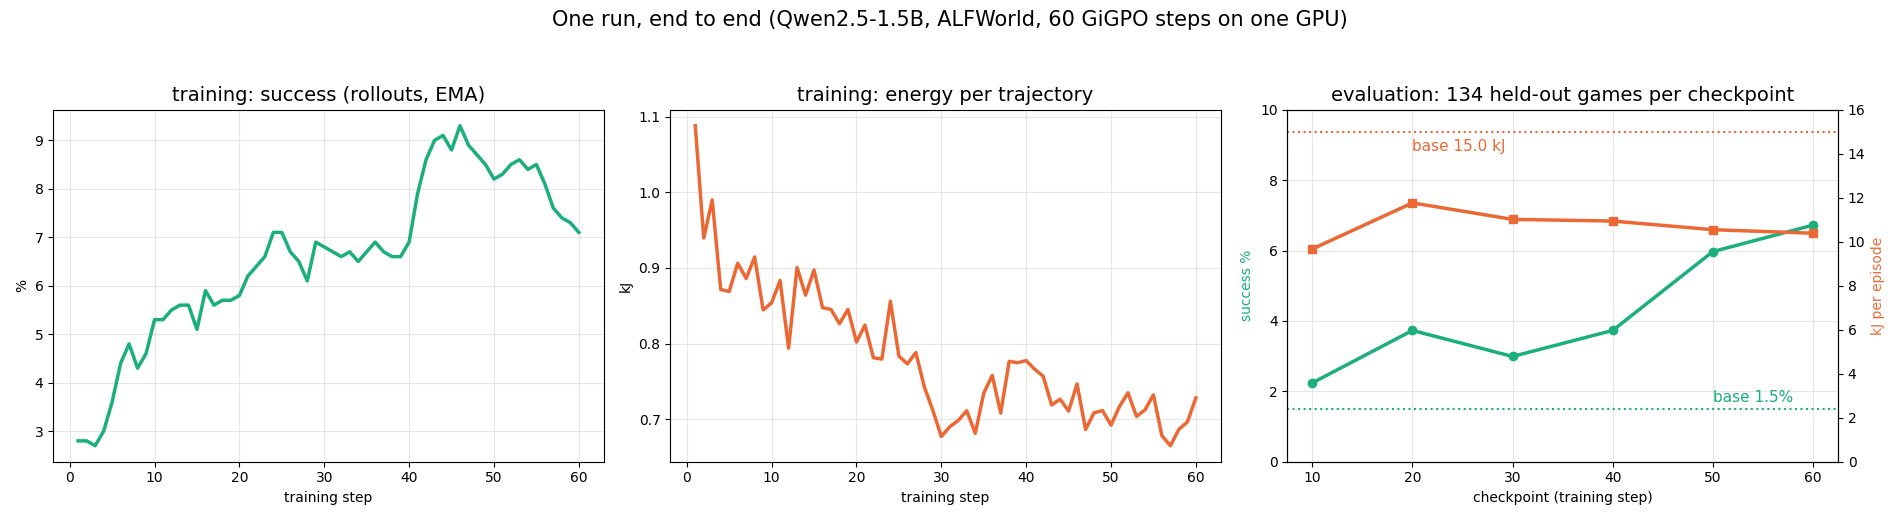
\includegraphics[width=0.98\textwidth]{figures/a2_run.png}\end{center}
\vspace{-0.4em}\small
Success $1.5\,\% \rightarrow 6.7\,\%$ while energy falls $15.0 \rightarrow 10.4$ kJ/episode
($-31\,\%$): the trained agent beats the untrained one \textbf{on both axes at once}.
\end{frame}

% -----------------------------------------------------------------------------
\begin{frame}{But the \emph{choice} collapsed: it always says ``mid''}
\begin{center}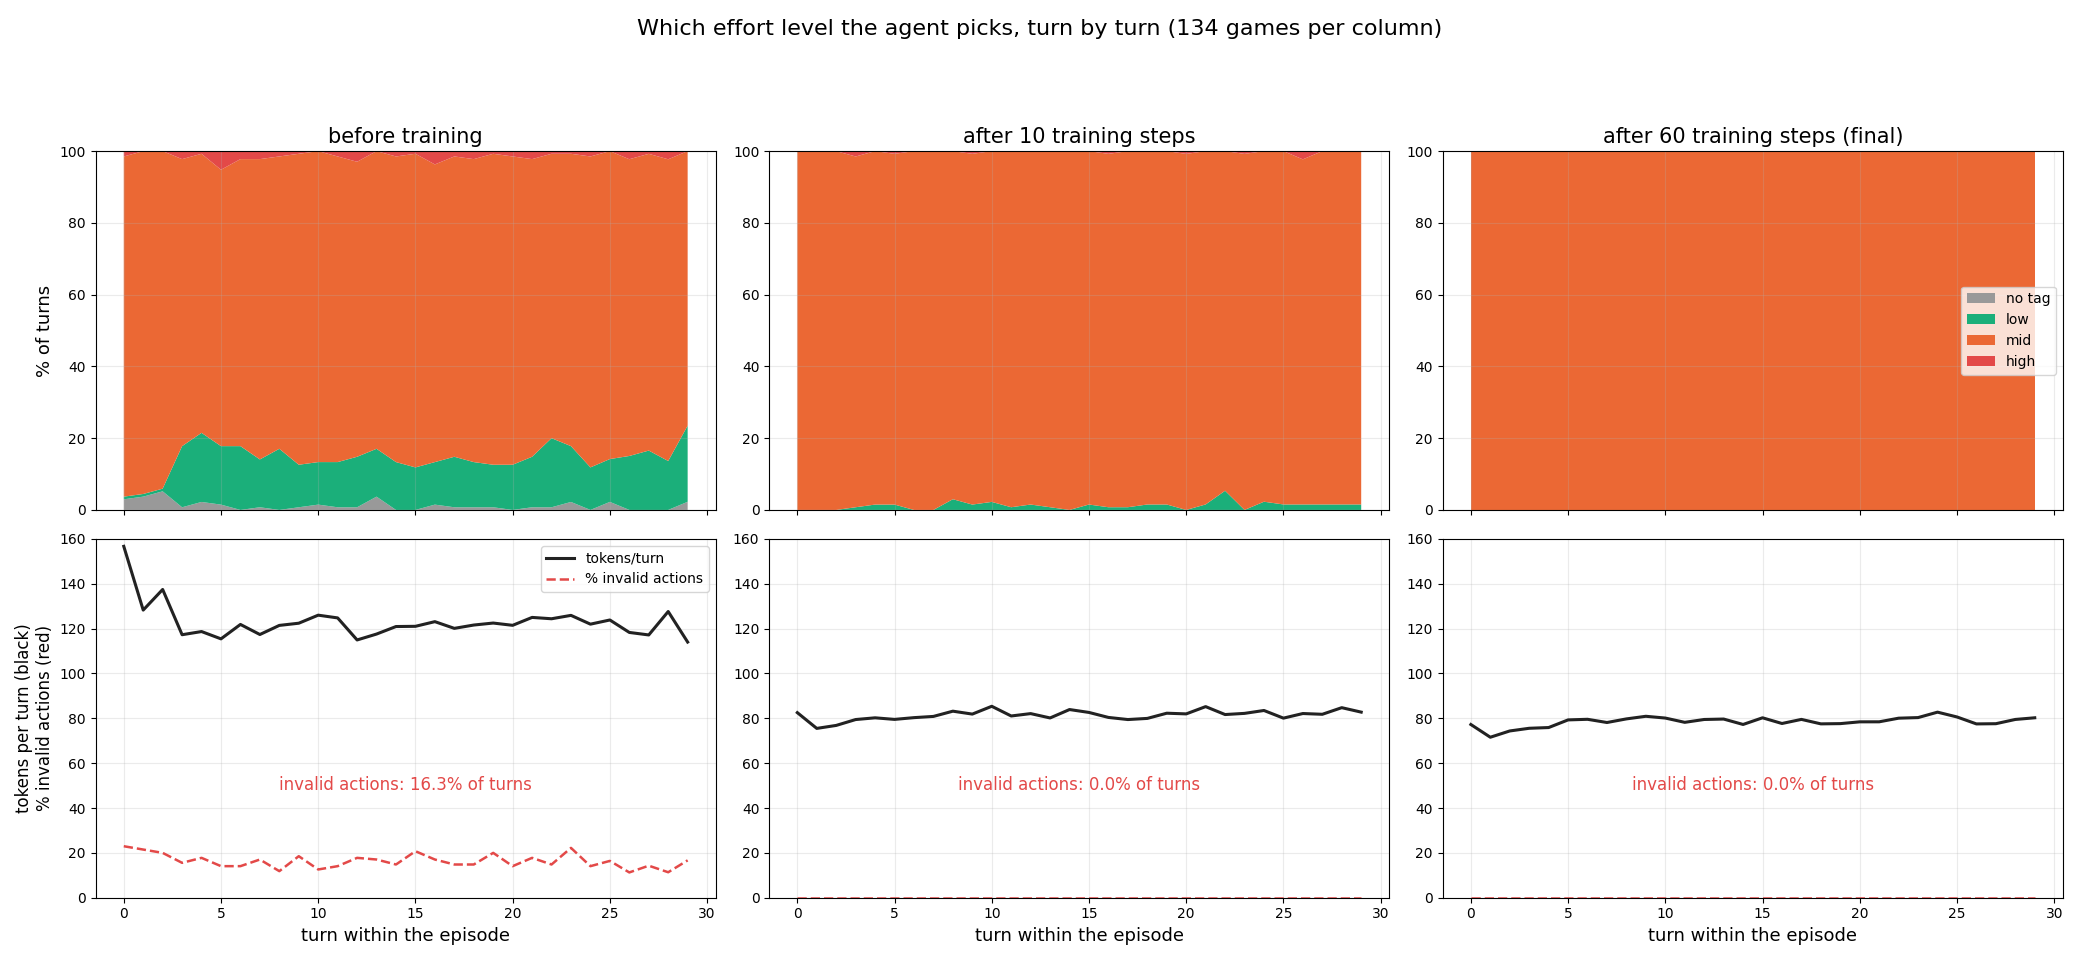
\includegraphics[width=0.82\textwidth]{figures/choice_evolution.png}\end{center}
\vspace{-0.5em}\small
Before training it picks levels erratically (and breaks the format in 16\,\% of turns);
after training it says \textbf{mid 100\,\% of the time} and just writes less. The energy saving
is real --- but it comes from brevity and format, \textbf{not from the decision we wanted}.
\end{frame}

% -----------------------------------------------------------------------------
\begin{frame}{Where the energy went --- and what's next}
\begin{center}\normalsize
\begin{tabular}{@{}lrr@{}}
\toprule
 & success & kJ/episode \\
\midrule
before training (base model) & 1.5\,\% & 15.0 \\
normal RL training (no energy term) & 3.7\,\% & 10.3 \\
\textbf{our modification (energy in the reward)} & \textbf{6.7\,\%} & \textbf{10.4} \\
\bottomrule
\end{tabular}
\end{center}
\vspace{0.3em}\small
\begin{itemize}\itemsep 0.4em
  \item Most of the saving comes from \textbf{training itself} (brevity + valid actions);
        the energy term didn't add savings --- because the agent stopped choosing.
  \item And the collapsed choice \textbf{leaves energy on the table}: forcing ``low'' on the
        trained agent keeps its 6.7\,\% success at \textbf{8.8 kJ} ($-16\,\%$).
  \item \textbf{Next (already training)}: make the choice itself matter --- put a price on the
        declared level, and show the agent its own consumption against a budget.
\end{itemize}
\vspace{0.2em}
{\footnotesize 134 held-out games per row, same GPU protocol; checkpoint 60 for both trained rows
(each run's best checkpoint tells the same story). Details, controls, and traces: appendix.}
\end{frame}

\appendix


% -----------------------------------------------------------------------------
\begin{frame}{Aug 12 asks: five closed with evidence; PES GM is today's decision}
\begin{center}\footnotesize
\begin{tabular}{@{}p{6.8cm}lp{5.6cm}@{}}
\toprule
\textbf{You asked (Aug 12)} & \textbf{Who} & \textbf{Now} \\
\midrule
Same GPU for every energy comparison & Yuanyuan & \textcolor{good}{\textbf{done}}, plus stronger: per-board J/token \emph{calibration} (four ``identical'' 3090s measured 4.0--6.4 J/token) \\
Turns free, not fixed at 5 & Yuanyuan & \textcolor{good}{\textbf{done}} --- turns are an outcome everywhere \\
Explain the long act segments & Yuanyuan & \textcolor{good}{\textbf{answered}}: a 2nd LLM call hitting its 200-token ceiling; env was never in it (backup) \\
Peak power in the idle period & Wenqi & \textcolor{good}{\textbf{answered}}: NVML power is a trailing average; probe now samples the instantaneous field too (backup) \\
RL with the action specified, success-only penalty & all & \textcolor{good}{\textbf{ran}}: 6 trained runs (30--60 steps), 27 evaluations of 134 games each \\
Context window into the action space & Wenqi & authority \textcolor{good}{\textbf{measured}} (F4, overnight): cutting history \emph{hurts} success and saves no energy --- context stays an observation at 1.5B \\
PES GM 2027 (Nov 10) & Yuanyuan & timeline slide at the end --- decision needed \\
\bottomrule
\end{tabular}
\end{center}
\end{frame}

% -----------------------------------------------------------------------------
\begin{frame}{Built: effort-as-action RL on Nautilus + a calibrated 134-game eval protocol}
\small
\begin{enumerate}\itemsep 0.45em
  \item \textbf{The full effort-as-action stack on NRP Nautilus}: the policy declares
        \texttt{<effort>low|mid|high</effort>} each turn; NVML energy reaches the reward
        (the June inert-penalty bug is closed \emph{with evidence}); LoRA-64 training fits a
        free-pool 24-GB A10. It took 8 attempts --- each failure advanced one stage
        (\texttt{python} shim, host-RAM, flash-attn, CUDA-OOM, LoRA) and is documented.
  \item \textbf{A verifiable evaluation protocol}: 134 out-of-distribution games per point,
        the exact training prompt (byte-identical templates), hardware energy counter,
        \textbf{per-board J/token calibration}, eviction-proof resume. 27 evaluations done.
  \item \textbf{Fixed-effort baselines (F1)} and the untrained reference points.
  \item Two bug classes found in \emph{our own} earlier pipeline and fixed: energy attribution
        was $\sim$uniform across trajectories; the energy meter could fail silently.
\end{enumerate}
\end{frame}

% -----------------------------------------------------------------------------
\begin{frame}{The mechanism: one turn --- three separate channels out of the same text}
\begin{center}
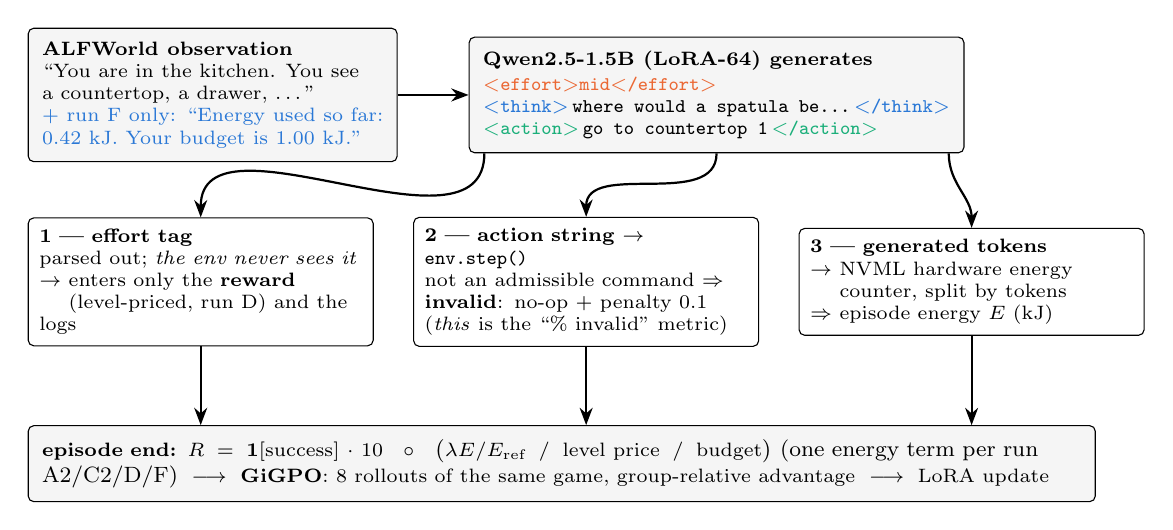
\begin{tikzpicture}[
  font=\scriptsize,
  box/.style={draw, rounded corners=2pt, align=left, inner sep=5pt},
  chan/.style={draw, rounded corners=2pt, align=left, inner sep=4pt, text width=4.1cm},
  arr/.style={-{Stealth[length=2.2mm]}, thick},
  node distance=4mm and 7mm]

\node[box, fill=black!4] (obs) {\textbf{ALFWorld observation}\\
  ``You are in the kitchen. You see\\ a countertop, a drawer, \ldots''\\
  \textcolor{acc}{+ run F only: ``Energy used so far:}\\
  \textcolor{acc}{0.42 kJ. Your budget is 1.00 kJ.''}};

\node[box, right=9mm of obs, fill=black!4] (gen) {\textbf{Qwen2.5-1.5B (LoRA-64) generates}\\[1pt]
  \texttt{\textcolor{mid}{\ab{effort}mid\ab{/effort}}}\\
  \texttt{\textcolor{acc}{\ab{think}}\,where would a spatula be\ldots\,\textcolor{acc}{\ab{/think}}}\\
  \texttt{\textcolor{good}{\ab{action}}\,go to countertop 1\,\textcolor{good}{\ab{/action}}}};

\node[chan, below=7mm of obs.south west, anchor=north west] (ceff)
  {\textbf{1 --- effort tag}\\ parsed out; \emph{the env never sees it}\\
   $\rightarrow$ enters only the \textbf{reward}\\ \phantom{$\rightarrow$} (level-priced, run D) and the logs};
\node[chan, right=5mm of ceff] (cact)
  {\textbf{2 --- action string} $\rightarrow$ \texttt{env.step()}\\
   not an admissible command $\Rightarrow$\\ \textbf{invalid}: no-op $+$ penalty 0.1\\
   (\emph{this} is the ``\% invalid'' metric)};
\node[chan, right=5mm of cact] (cnrg)
  {\textbf{3 --- generated tokens}\\ $\rightarrow$ NVML hardware energy\\
   \phantom{$\rightarrow$} counter, split by tokens\\ $\Rightarrow$ episode energy $E$ (kJ)};

\node[box, below=10mm of ceff.south west, anchor=north west, fill=black!4, text width=13.2cm] (rew)
  {\textbf{episode end:} $R=\mathbf{1}[\text{success}]\cdot 10 \;\circ\;
    \big(\lambda E/E_{\text{ref}} \;/\; \text{level price} \;/\; \text{budget}\big)$
   {\footnotesize (one energy term per run A2/C2/D/F)}
   \;$\longrightarrow$\; \textbf{GiGPO}: 8 rollouts of the same game, group-relative advantage
   \;$\longrightarrow$\; LoRA update};

\draw[arr] (obs) -- (gen);
\draw[arr] (gen.south west) ++(2mm,0) to[out=-90,in=90] (ceff.north);
\draw[arr] (gen.south) to[out=-90,in=90] (cact.north);
\draw[arr] (gen.south east) ++(-2mm,0) to[out=-90,in=90] (cnrg.north);
\draw[arr] (ceff.south) -- (ceff.south |- rew.north);
\draw[arr] (cact.south) -- (cact.south |- rew.north);
\draw[arr] (cnrg.south) -- (cnrg.south |- rew.north);
\end{tikzpicture}
\end{center}
\vspace{-0.2em}\scriptsize
Independent channels: the \textbf{level} is judged by the reward, the \textbf{action} by the
environment, the \textbf{energy} by hardware --- ``\% invalid'' is channel 2 only, unrelated to the effort tag.
\end{frame}

% -----------------------------------------------------------------------------
\begin{frame}{F1: energy obeys the knob --- 10.7 $<$ 12.0 $<$ 13.0 kJ (low/mid/high), base free = 15.0}
\begin{columns}[T]
\column{0.46\textwidth}
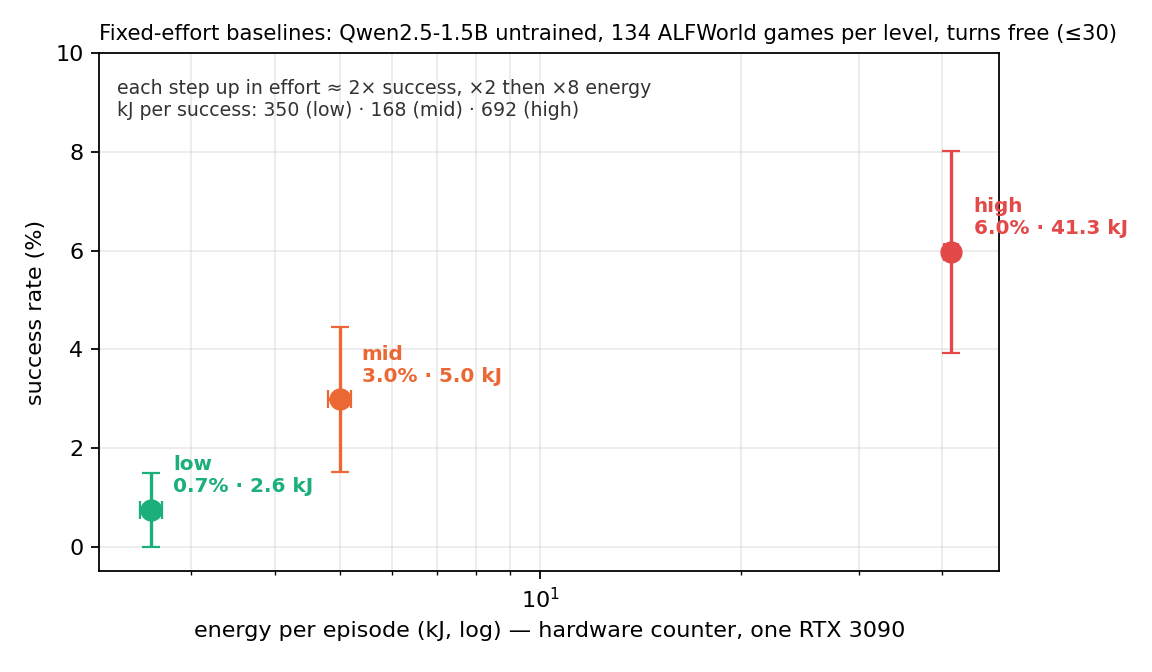
\includegraphics[width=\linewidth]{figures/f1_success_vs_energy.png}
\column{0.54\textwidth}\scriptsize
\vspace{0.4em}
\begin{tabular}{@{}lrrrr@{}}
\toprule
base + forced effort & success & kJ/ep & tok/turn \\
\midrule
low  & 0.8\,\% & 10.7 & 87 \\
mid  & 1.5\,\% & 12.0 & 98 \\
high & 1.5\,\% & 13.0 & 107 \\
free (no forcing) & 1.5\,\% & \textbf{15.0} & 123 \\
\bottomrule
\end{tabular}

\vspace{0.7em}
Energy orders \textbf{low $<$ mid $<$ high} on full episodes; the free base is the most
expensive of all (long, 16\,\% format-broken turns). Success is indistinguishable at this
model scale --- important later.

\vspace{0.5em}
{\tiny 134 games each, $\leq$30 turns, model decides length, RTX 3090, hardware counter.
Left figure: the single-call profiler protocol (F1); table: the training-prompt protocol.}
\end{columns}
\end{frame}

% -----------------------------------------------------------------------------
\begin{frame}{Experiment 1 --- one config, one control: does the energy penalty do anything?}
\small
\textbf{The question}: if the reward pays for saving energy, does the agent use its effort knob?
\vspace{0.4em}
\begin{center}\footnotesize
\begin{tabular}{@{}lll@{}}
\toprule
 & \textbf{A2 (treatment)} & \textbf{B2 (control)} \\
\midrule
reward & $R=\mathbf{1}[\text{success}]\cdot 10\cdot\max(0,1-\lambda E/E_{\text{ref}})$ & same, with $\lambda=0$ (no energy term) \\
$\lambda$ & 0.5 & 0 \\
\bottomrule
\end{tabular}
\end{center}
\vspace{0.4em}
\textbf{Everything else identical}: Qwen2.5-1.5B + LoRA-64, GiGPO (8 rollouts/game,
128 trajectories/step), lr 3e-6, no KL, \textbf{60 steps} on one free-pool GPU,
checkpoint every 5 steps. Evaluation: every 10th checkpoint $\times$ \textbf{134
out-of-distribution games}, byte-identical prompt, board-calibrated hardware joules.
\vspace{0.4em}

$\Rightarrow$ three results, next three slides: the Pareto plot, the choice dynamics, the raw traces.
{\scriptsize (An earlier weak-recipe batch A/B/A$'$ at lr 1e-6 + KL and $\lambda\in\{0,0.5,1.5\}$
reached the same verdict --- backup.)}
\end{frame}

% -----------------------------------------------------------------------------
\begin{frame}{Exp.\ 1, result A: training cuts energy 32\,\% at better success --- but so does $\lambda{=}0$}
\begin{columns}[T]
\column{0.5\textwidth}
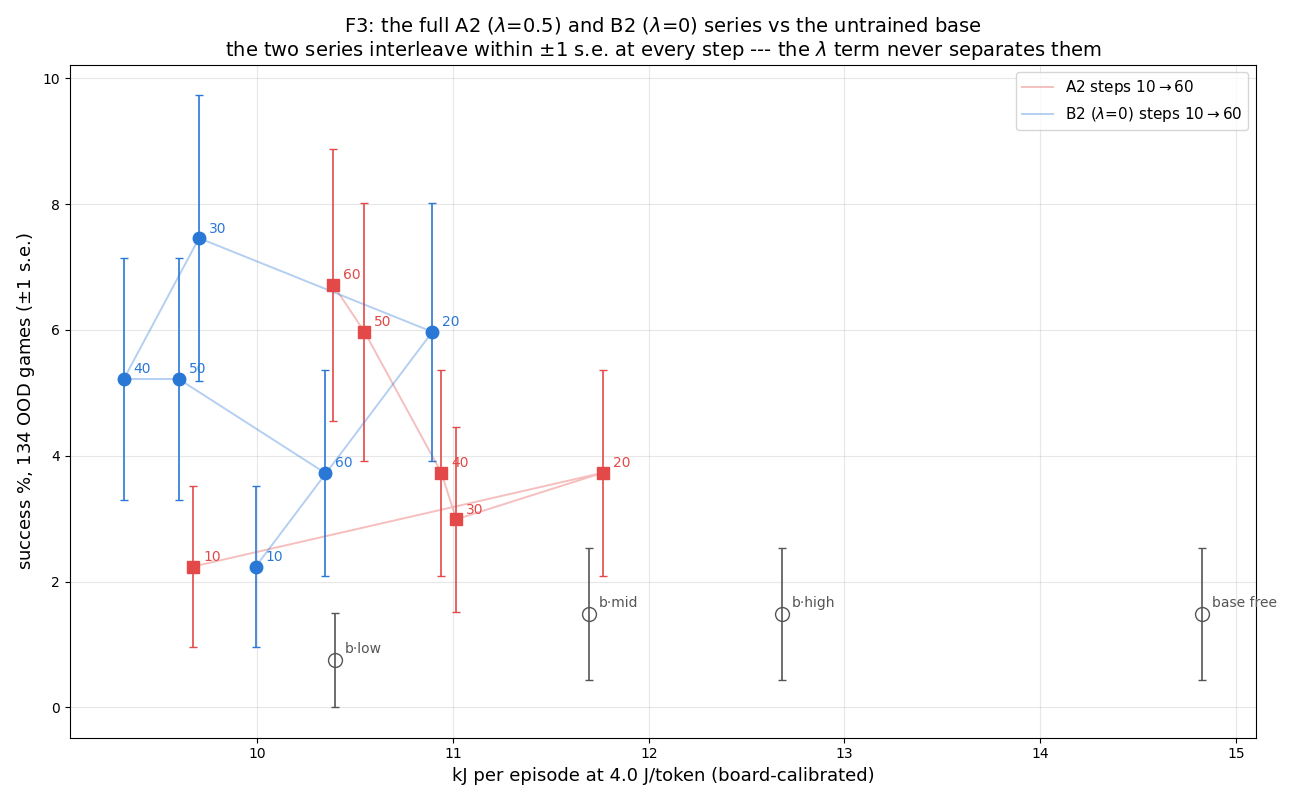
\includegraphics[width=\linewidth]{figures/f3_pareto.png}
\column{0.5\textwidth}\small
\begin{itemize}\itemsep 0.4em
  \item Every trained checkpoint: 15.0 $\rightarrow$ \textbf{10.2--10.5 kJ/episode}
        (123 $\rightarrow$ 83--87 tokens/turn), success preserved.
  \item With the stronger recipe (A2, 60 steps) success also \textbf{rises}:
        1.5\,\% $\rightarrow$ \textbf{6.7\,\%} while energy falls 12.1 $\rightarrow$ 10.4 kJ ---
        the trained point \emph{dominates} base on both axes.
  \item But: identical at $\lambda = 0$, $0.5$, $1.5$ --- and the full $\lambda{=}0$ series (B2,
        overnight) \textbf{seals it}: B2 peaks at \textbf{7.5\,\% / 9.7 kJ} (step 30), equal-or-better
        than $\lambda{=}0.5$'s best point (6.7\,\% / 10.4 kJ, step 60).
        \textbf{The energy term did not cause it} --- GiGPO itself does.
\end{itemize}
\end{columns}
\end{frame}

% -----------------------------------------------------------------------------
\begin{frame}{Exp.\ 1, result B: the choice collapses --- 133/134 episodes vary levels $\rightarrow$ 0/134}
\begin{center}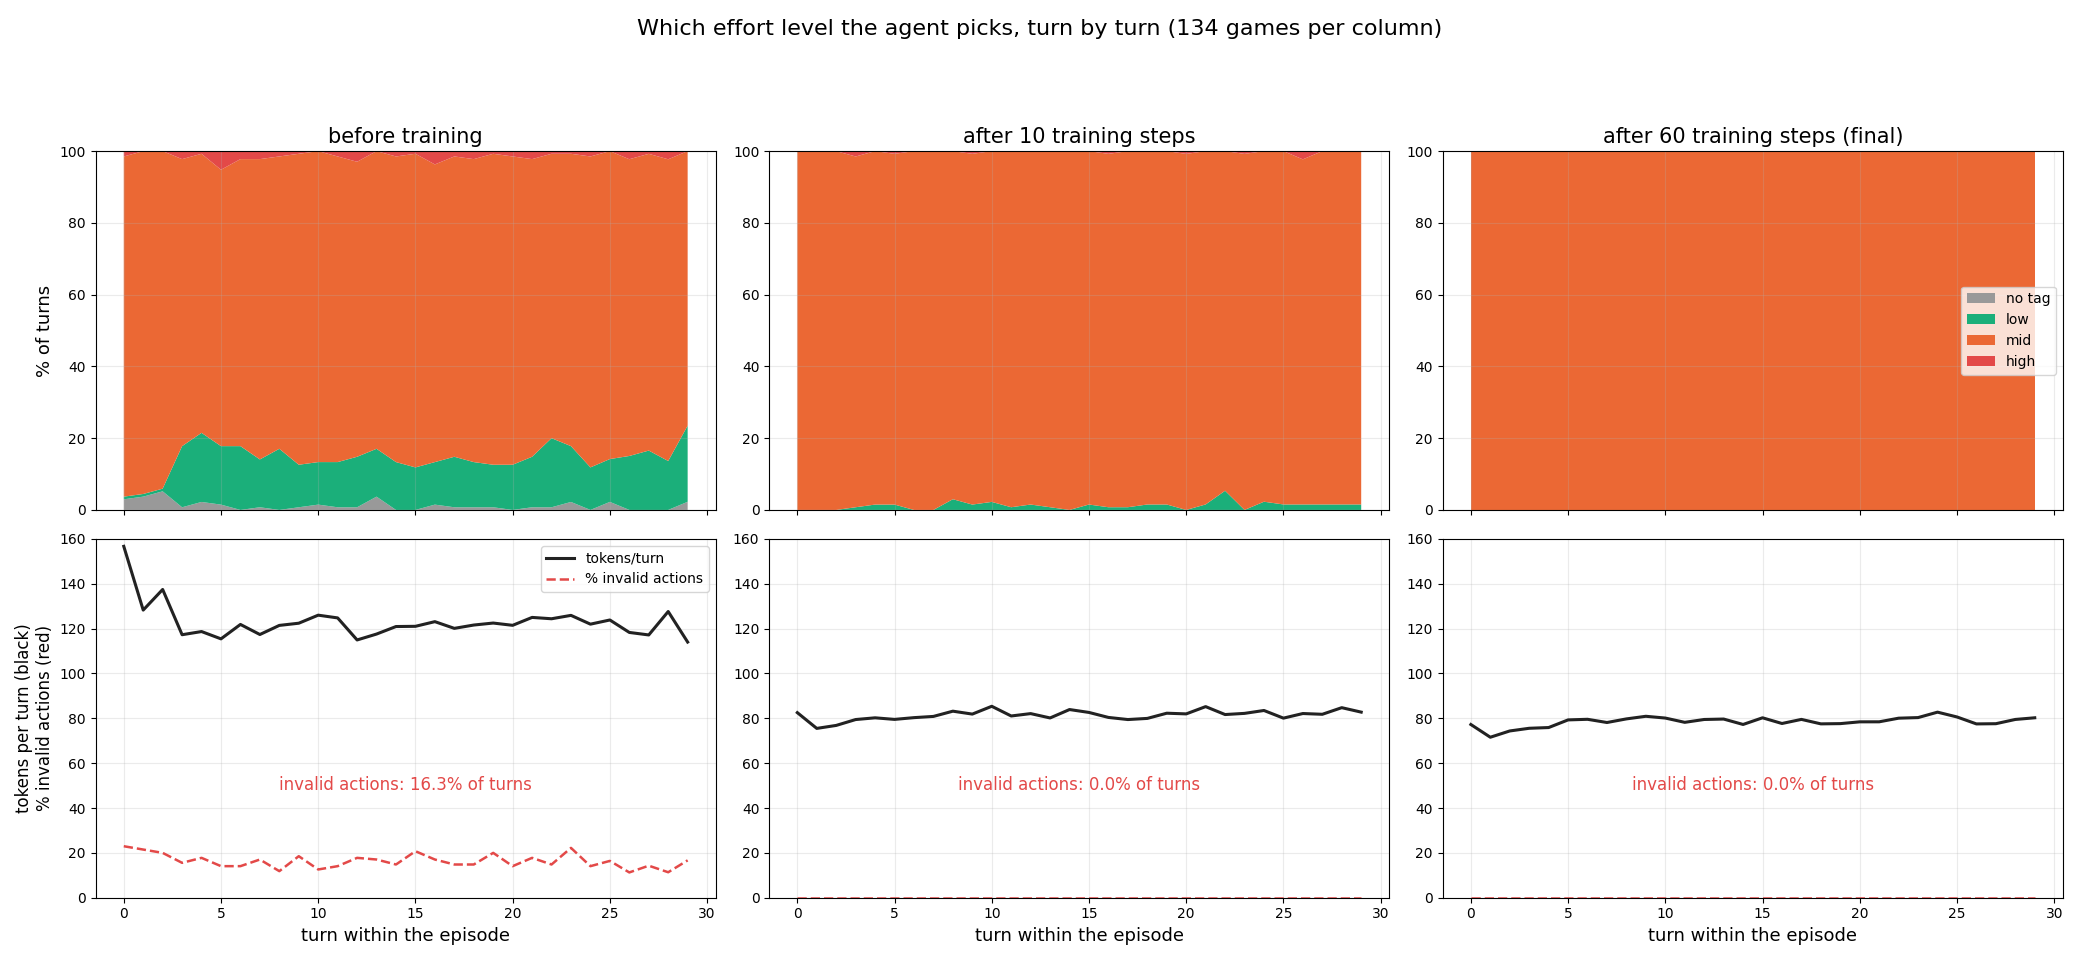
\includegraphics[width=0.86\textwidth]{figures/choice_evolution.png}\end{center}
\vspace{-0.6em}\scriptsize
Episodes using more than one effort level: base \textbf{133/134} (scatter + 16\,\% broken format)
$\rightarrow$ A2@10 \textbf{43/134} $\rightarrow$ A2@60 \textbf{0/134}. Training \emph{removes}
variation: it learns format and brevity, converging to ``always mid, short'' --- the trace
decomposition shows 100\,\% of the energy drop is \textbf{within-mid shortening}
(125$\rightarrow$83 tok), 0\,\% is level switching, 0\,\% is shorter episodes.
\end{frame}

% -----------------------------------------------------------------------------
\begin{frame}{Exp.\ 1, the traces: the rambling dies ($-35\,\%$/turn); the decision never appears}
\begin{columns}[T]
\column{0.5\textwidth}
{\small \textbf{Base (untrained)} --- ``put a clean spatula in a drawer'', turn 1:}\\[0.2em]
{\scriptsize\ttfamily
\textcolor{mid}{\ab{effort}mid\ab{/effort}}\\
In the current situation, I have a spatula but no clean spatula. To find a clean
spatula, I would first check if there is a dirty spatula on any of the countertops,
sinks, stoves, etc., then wash it with water from the sinkbasin before placing it
back into the drawer. However, since I don't know which object currently has the
spatula, I will simply go to the sinkbasin [\ldots]\\
\textcolor{acc}{\ab{think}} I am looking for a clean spatula [\ldots]}
\column{0.5\textwidth}
{\small \textbf{A2@60 (trained)} --- same task, turn 1:}\\[0.2em]
{\scriptsize\ttfamily
\textcolor{mid}{\ab{effort}mid\ab{/effort}}\\
\textcolor{acc}{\ab{think}} The spatula must be somewhere in the kitchen [\ldots]
The most likely places would be on the countertops, in the drawers, or in the
cabinets. \textcolor{acc}{\ab{/think}}\\
\textcolor{good}{\ab{action}go to countertop 1\ab{/action}}}\\[0.6em]
{\small The rambling preamble is gone; think is tight; straight to a valid action.}
\end{columns}
\vspace{0.5em}\scriptsize
Across the 3 sampled games (same board, 4.3 J/tok): median \textbf{483 $\rightarrow$ 314
chars/turn} ($-35\,\%$), \textbf{14.9 $\rightarrow$ 8.3 kJ/episode}; both solve the same game,
A2 in 13 turns. But the \emph{tag}: base scatters 66 mid / 20 low / 3 high (confusion, not
strategy) $\rightarrow$ A2 emits \textbf{mid 73/73 times}. Training deleted the waste
\emph{inside} the level --- it did not learn to \emph{choose} the level.
\end{frame}

% -----------------------------------------------------------------------------
\begin{frame}{Experiment 2 --- force each level on the trained policy: do its choices matter?}
\small
\textbf{The question}: is the learned ``always mid'' actually a good choice?
\textbf{Setup}: the same A2@60 checkpoint, 134 games per row; the only change is a forced
\texttt{<effort>} prefix in the assistant turn. If free choice $\succ$ every forced level,
the choices carry information.
\vspace{0.4em}
\begin{center}\footnotesize
\begin{tabular}{@{}llll@{}}
\toprule
config & success & kJ/episode & \\
\midrule
A2@60, its own choice (= always mid) & 6.7\,\% & 10.4 & \\
A2@60 \textbf{forced low} & \textbf{6.7\,\%} & \textbf{8.8} & \textcolor{bad}{same success, $-16\,\%$ energy} \\
A2@60 forced mid / forced high & \multicolumn{2}{l}{running (tonight)} & \\
\bottomrule
\end{tabular}
\end{center}
\vspace{0.4em}
\textbf{Answer so far: no.} A fixed ``low'' matches the trained policy's success at 16\,\% less
energy --- the learned choice \textbf{leaves energy on the table}. This is the precise gap the
next round of training (next slide) has to close.
\end{frame}

% -----------------------------------------------------------------------------
\begin{frame}{Five causes of the collapse --- each one has an experiment running against it}
\begin{center}\footnotesize
\begin{tabular}{@{}p{5.6cm}p{5.3cm}l@{}}
\toprule
\textbf{cause} & \textbf{fix} & \textbf{status} \\
\midrule
Success-gated reward touches only $\sim$5\,\% of trajectories $\Rightarrow$ almost no energy gradient & additive reward: charge \emph{every} trajectory (ARES's fail-faster risk is the point of the ablation) & runs C/C2 training \\
Choosing a level has no price of its own & \textbf{level-priced} reward: low free, mid $-c$, high $-3c$ per turn & run D training \\
Energy is invisible to the policy (reward-only, never observed) & \textbf{budget in the observation} (June's budget-conditioning, reborn) & run F training \\
GiGPO groups contain no level counterfactuals (all 8 rollouts pick mid) & forced-level exploration within groups (2 low / 4 free / 2 high) & designed, next \\
At 2--7\,\% success the levels barely change outcomes --- there is little ``when'' to learn & more data / steps / 7B on B200 & lever known \\
\bottomrule
\end{tabular}
\end{center}
\vspace{0.2em}\footnotesize
Plus the \textbf{decision test} --- first result overnight: A2@60 \emph{forced to low} scores
\textbf{6.7\,\% at 8.8 kJ} vs its free choice \textbf{6.7\,\% at 10.4 kJ}: same success,
$-16\,\%$ energy --- always-mid \textbf{leaves energy on the table} (mid/high still running).
\end{frame}

% -----------------------------------------------------------------------------
\begin{frame}{Now training: three targeted fixes, one per diagnosed cause}
\begin{center}\small
\begin{tabular}{@{}lp{5.6cm}p{5.2cm}@{}}
\toprule
run & the one change vs Experiment 1 & the failure it attacks \\
\midrule
C2 & \textbf{additive} reward $R=\text{task}-\lambda E$, every trajectory pays & energy gradient reached only $\sim$5\,\% of trajectories \\
D & \textbf{level-priced}: low free, mid $-c$, high $-3c$ per turn & the declaration itself never cost anything \\
F & \textbf{budget line in every observation} (``Energy used so far: X kJ / budget 1 kJ'') & the policy could never \emph{see} its energy \\
\bottomrule
\end{tabular}
\end{center}
\vspace{0.4em}\small
All three: same recipe/scale as Experiment 1, 60 steps, checkpoints on the PVC, monitored.
In the eval queue: Experiment 2's forced mid/high + F5 (does the \emph{untrained} model react
to a stated budget?). Next knob after these verdicts: \textbf{learning to stop} --- 95--99\,\%
of episodes burn all 30 turns while successes finish in 15--22.
\end{frame}

% -----------------------------------------------------------------------------
\begin{frame}{Measurement: four ``identical'' 3090s differ 60\,\% --- calibrate boards, count tokens}
\small
\begin{enumerate}\itemsep 0.5em
  \item \textbf{``Same GPU model'' is not enough}: four RTX 3090s (same 350-W limit) measured
        4.0--6.4 J/token for identical policies. Every evaluation now runs a 1-minute per-board
        calibration; energy is reported at a 4.0 J/token reference. Raw cross-board kJ
        comparisons are invalid --- ours and anyone's.
  \item \textbf{Tokens/episode is the hardware-free energy currency} of the policy; joules are
        tokens $\times$ a board property.
  \item \textbf{Attribution $\neq$ measurement}: batched training energy is split by generated
        tokens (we fixed a bug where it was $\sim$uniform); offline eval measures single episodes.
  \item NVML's power reading is a $\sim$1-s trailing average --- peak-power claims need
        \texttt{NVML\_FI\_DEV\_POWER\_INSTANT} (in the probe now).
\end{enumerate}
\end{frame}

% -----------------------------------------------------------------------------
\begin{frame}{Five claims stand on 134-game evidence; three verdicts land this week}
\footnotesize
\textbf{Claimable now, with 134-game evidence:}
\begin{itemize}\itemsep 0.15em
  \item The effort knob has real authority (F1: low $<$ mid $<$ high in energy).
  \item RL training yields \textbf{$-32\,\%$ energy at equal-or-better success} (A2@60 dominates base).
  \item Success-gated multiplicative rewards, $\lambda \in \{0, 0.5, 1.5\}$, do \emph{not} make
        the policy exercise the knob --- and the full B2 series (overnight) confirms
        $\lambda$ \textbf{never separates} from the $\lambda{=}0$ control.
  \item Context is not a useful knob at 1.5B (F4): truncating history costs success, saves no energy.
  \item First decision-test point: forced-low ties free choice on success at $-16\,\%$ energy
        --- the trained ``always mid'' \textbf{demonstrably leaves energy on the table}.
\end{itemize}
\vspace{0.3em}
\textbf{One result away (this week):}
\begin{itemize}\itemsep 0.15em
  \item Decision test, forced mid/high $\Rightarrow$ completes the ``do choices matter'' verdict.
  \item F5 $\Rightarrow$ does the untrained model react to a stated budget zero-shot?
  \item D / F $\Rightarrow$ does pricing the decision, or showing the budget, create real
        effort selection --- the claim we actually want.
\end{itemize}
\end{frame}

% -----------------------------------------------------------------------------
\begin{frame}{Asks: PES GM go/no-go (Oct), one reliable 48-GB GPU, your read on the 3 interventions}
\begin{enumerate}\itemsep 0.7em
  \item \textbf{PES GM 2027 (deadline Nov 10)}: with today's material the paper is
        ``knob authority + verified measurement methodology + RL saves 32\,\% + diagnosed
        limits of reward shaping''. Is that the paper, or do we hold for the decision result?
        Site opens Oct 6 --- decision by early October.
  \item \textbf{Compute}: everything above ran on free-pool scraps (A10/3090, 8 failed attempts
        to fit 24 GB, evictions, two PVC-full incidents). One reliable 48-GB+ GPU --- B200 slot
        or a quota grant --- multiplies iteration speed; the 7B experiments need it.
  \item \textbf{Design opinion}: of the three interventions now training (charge everything /
        price the level / show the budget), which failure or success would change your view of
        the approach?
  \item Meeting cadence: results now arrive every 24--48 h; propose a short weekly check-in.
\end{enumerate}
\end{frame}

% =============================================================================


\begin{frame}{Backup --- the full run matrix (9 runs, 4 reward families)}
\begin{center}\footnotesize
\begin{tabular}{@{}llllll@{}}
\toprule
run & reward & $\lambda$ & recipe & steps & status \\
\midrule
A  & multiplicative (success-gated) & 0.5 & lr 1e-6 + KL & 30 & done + evaluated \\
B  & --- (control) & 0 & lr 1e-6 + KL & 30 & done + evaluated \\
A$'$ & multiplicative & 1.5 & lr 1e-6 + KL & 30 & done + evaluated \\
A2 & multiplicative & 0.5 & \textbf{lr 3e-6, no KL} & 60 & done + evaluated \\
B2 & --- (control) & 0 & lr 3e-6, no KL & 60 & done + evaluated \\
C / C2 & \textbf{additive} (all trajectories) & 1.0 & 1e-6 / 3e-6 & 30 / 60 & training now \\
D  & \textbf{level-priced} (the decision costs) & --- & 3e-6 & 60 & training now \\
F  & multiplicative + \textbf{budget in the observation} & 0.5 & 3e-6 & 60 & training now \\
\bottomrule
\end{tabular}
\end{center}
\vspace{0.3em}\small
Reward forms: multiplicative $R=\mathbf{1}[\text{success}]\cdot 10\cdot\max(0,1-\lambda E/E_{\text{ref}})$;
additive $R=\text{task}-\lambda E$; level-priced $R=\text{task}-c\cdot\{0,1,3\}_{\text{declared level}}$;
run F adds ``\texttt{Energy used so far: X kJ. Your budget is 1.00 kJ.}'' to every observation.
\end{frame}


\begin{frame}{Backup --- F2 training curves, batch 1 (λ invisible at lr 1e-6)}
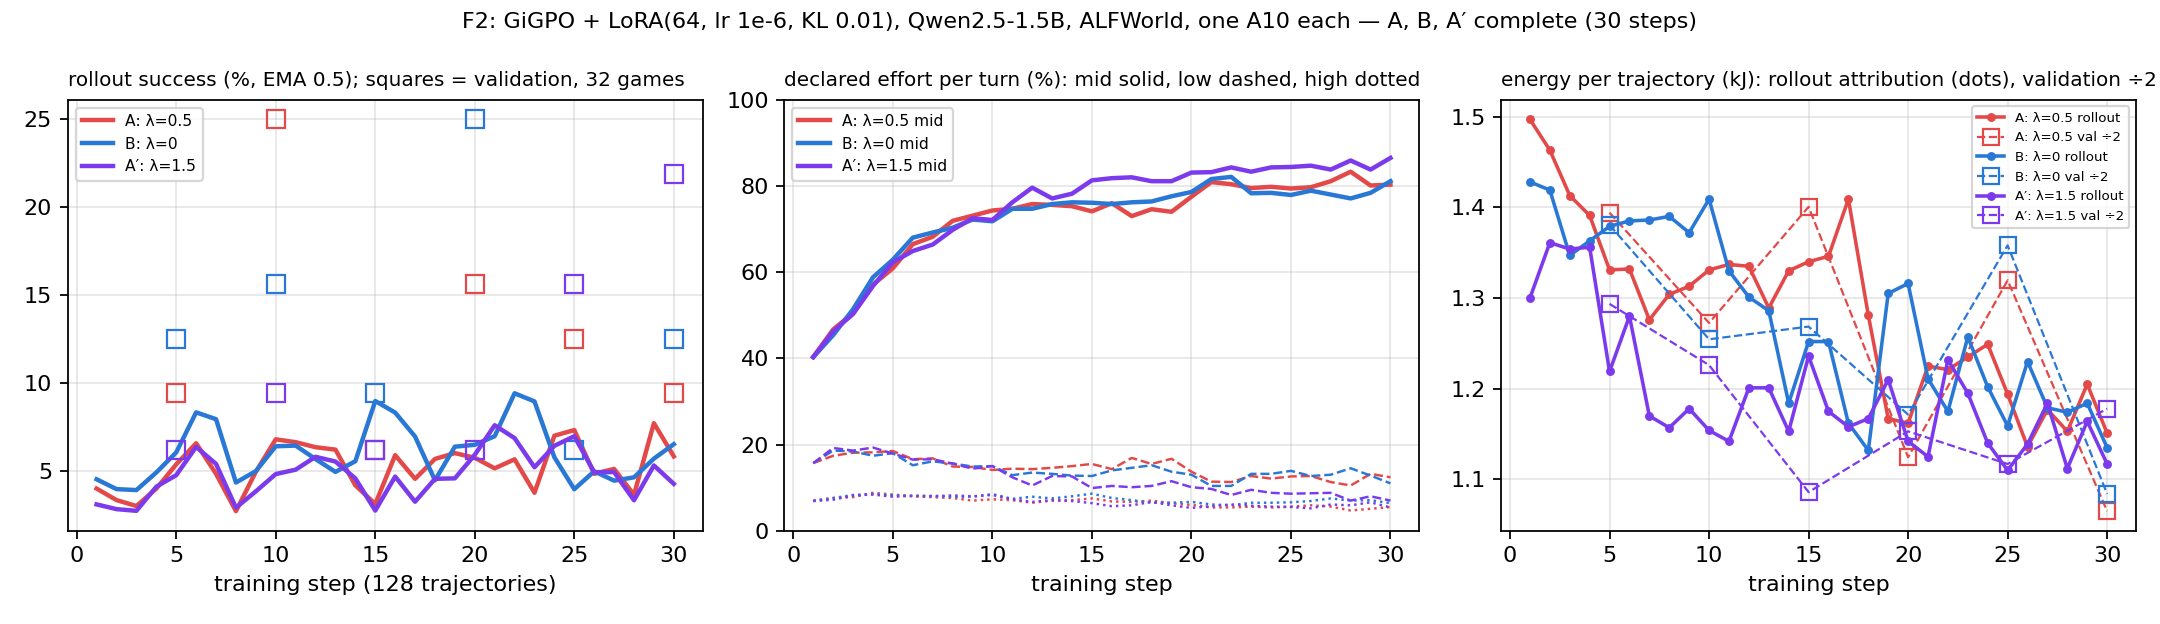
\includegraphics[width=\textwidth]{figures/f2_training_curves.png}
\end{frame}

\begin{frame}{Backup --- F2 batch 2 (lr 3e-6, no KL): success finally trends up}
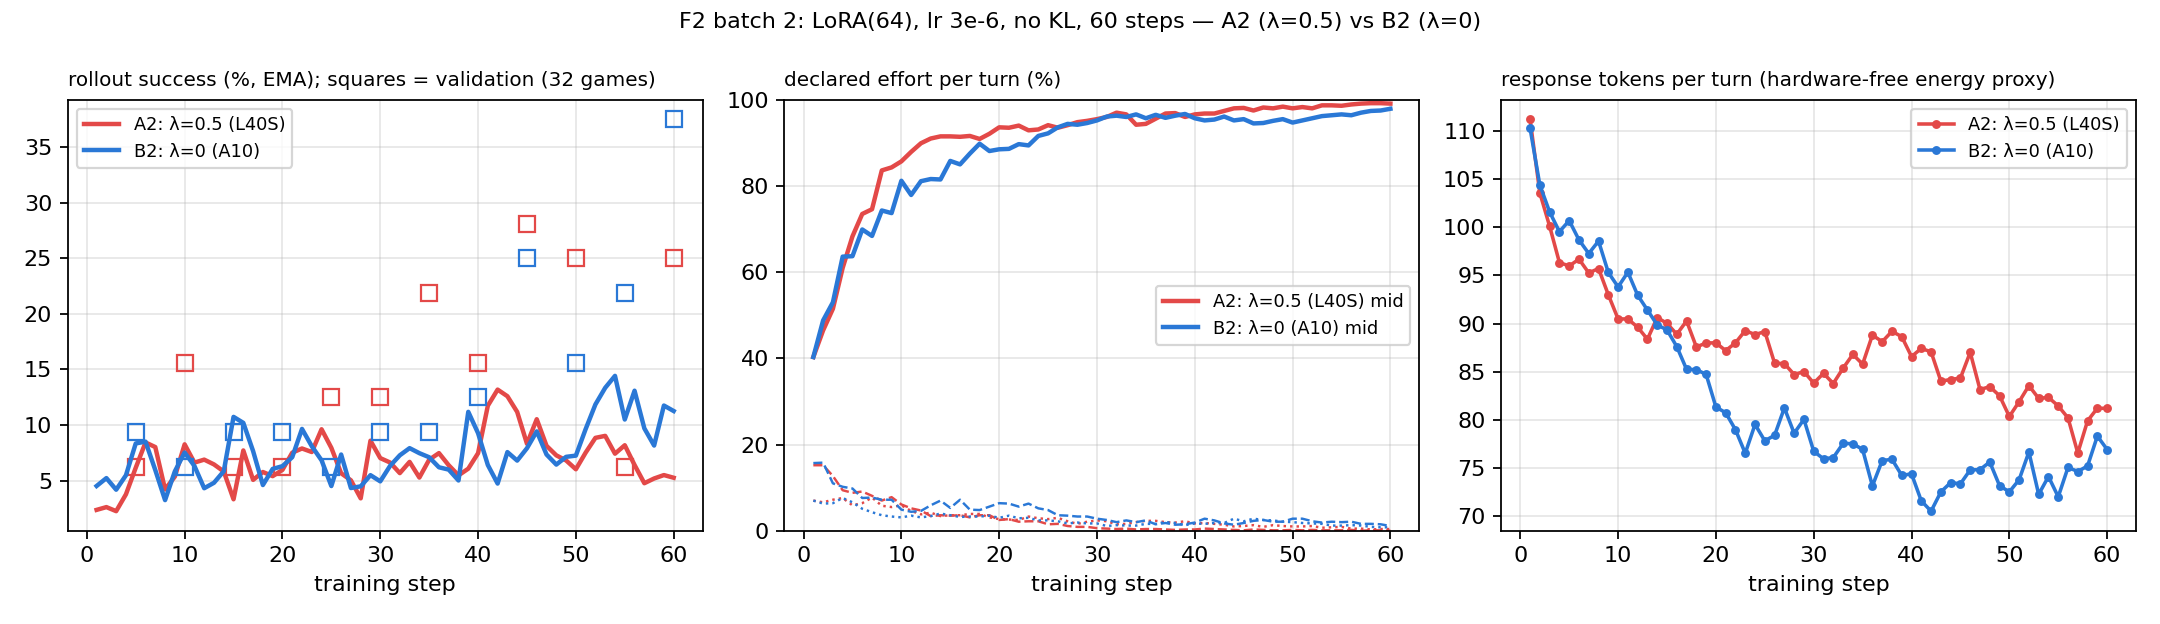
\includegraphics[width=\textwidth]{figures/f2_batch2_curves.png}
\vspace{-0.2em}\scriptsize
Validation (32 games, noisy): A2 6 $\rightarrow$ 25\,\%, B2 9 $\rightarrow$ 37\,\% by step 60;
tokens/turn 111 $\rightarrow$ 77--81. The 134-game evaluation of both series is the running arbiter.
\end{frame}

\begin{frame}{Backup --- answers owed from Aug 12}
\begin{columns}[T]
\column{0.55\textwidth}
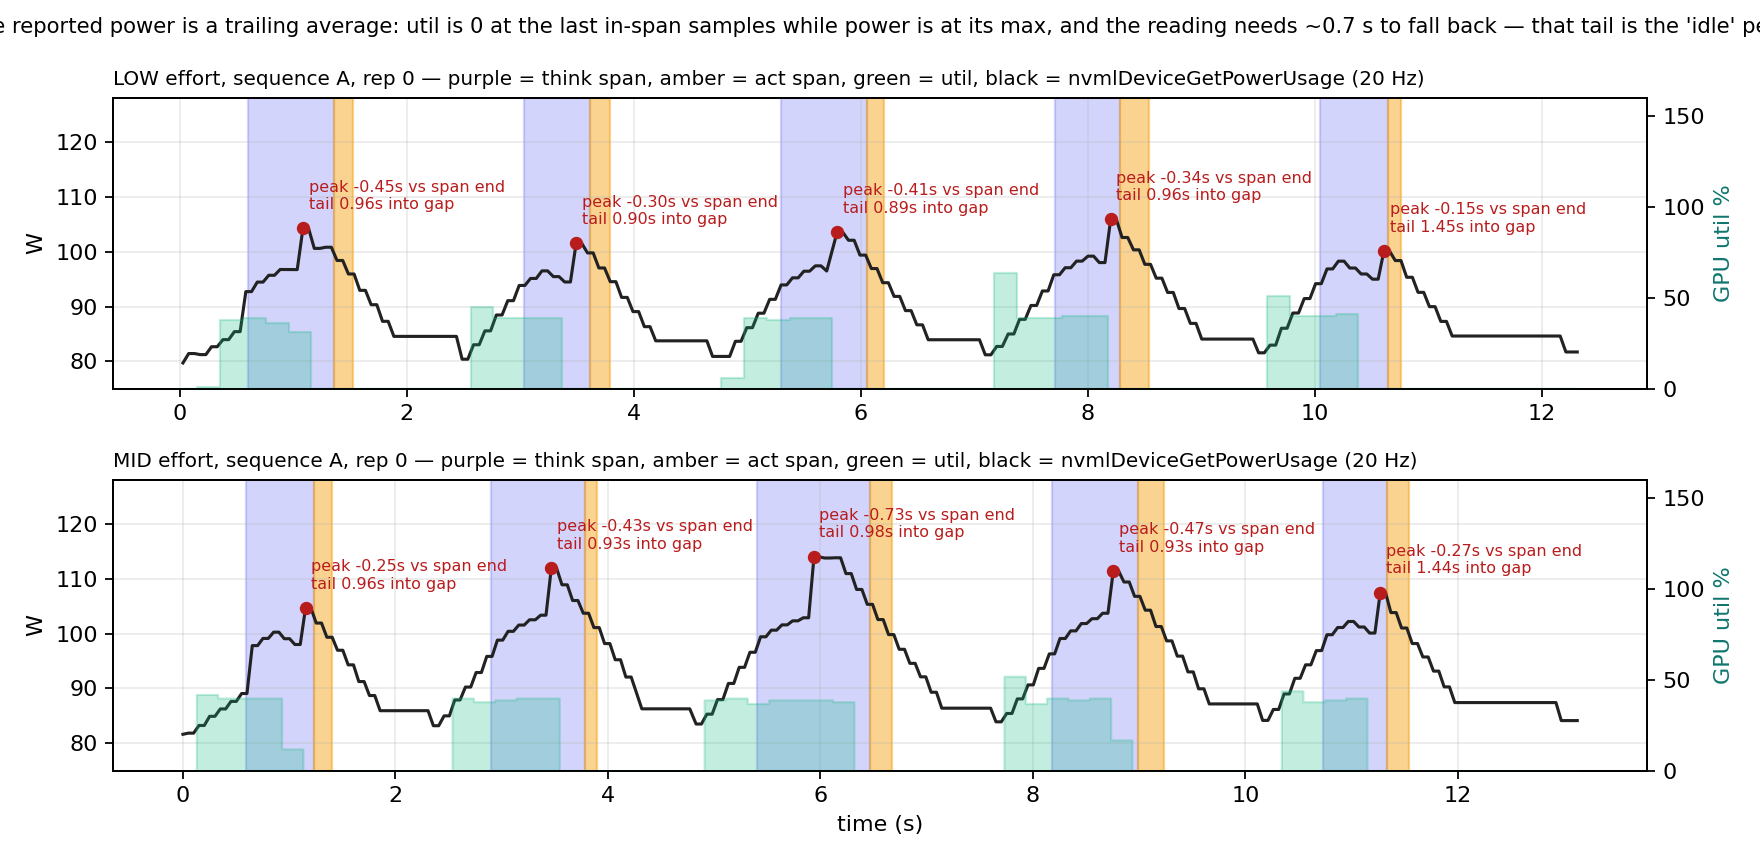
\includegraphics[width=\linewidth]{figures/peak_lag_low_mid.png}
\column{0.45\textwidth}\scriptsize
\textbf{A3, long act segments}: the Aug-12 profiler made a second LLM call per turn
(\texttt{...Action:}, ceiling 200); ``think thoroughly'' kept writing past \texttt{Action:} until
cut off. \texttt{env.step()} was outside every span. Fixed: single call, action parsed.

\vspace{0.5em}
\textbf{A4, peak in idle}: \texttt{nvmlDeviceGetPowerUsage} is a trailing average ($\sim$1 s);
utilization reads 0 while the reported power still peaks, and the decay tail (0.9--1.4 s) lands in
the unshaded gap. Joules (hardware counter) unaffected; probe now records the instantaneous field.
\end{columns}
\end{frame}

\begin{frame}{Backup --- ops on shared free-pool infrastructure (why this took 8 attempts)}
\scriptsize
\begin{tabular}{@{}llp{7.4cm}@{}}
\toprule
\# & failed at & lesson (all encoded in the Jobs now) \\
\midrule
1 & install & vLLM image has no \texttt{python} binary $\rightarrow$ shim \\
2--3 & env init & 256 ALFWorld processes OOM at 28/96 Gi host RAM $\rightarrow$ 160 Gi, 32 val envs \\
4 & model init & \texttt{flash\_attn} not in the image $\rightarrow$ prebuilt wheel \\
4--6 & actor update & full-FT Adam on 1.5B $>$ 24 GB $\rightarrow$ free vLLM cache, micro-batch, finally \textbf{LoRA-64} \\
7--8 & --- & training runs; evictions resume from checkpoints; logs mirrored to the PVC \\
\bottomrule
\end{tabular}
\vspace{0.5em}

Plus: 6-h bare-pod reap (run everything as Jobs), two PVC-full incidents (now 300 Gi + trim rule),
pod evictions during eval (resumable per game). Nautilus provided $\sim$470 free-pool GPUs on paper
and zero for six hours when we started.
\end{frame}

\end{document}
